% GLOBAL TODO LIST

% TODO: Fragezeichen suchen
% TODO: Proofread Kapitel 4 (Architekturen)
% TODO: schön machen

%\documentclass[pdftex,10pt,a4paper,twoside,openright]{scrreprt}
%\documentclass[pdftex,10pt,a4paper,twoside,openright]{scrbook} %12pt is offiziell
\documentclass[%pdftex,
	12pt,
	a4paper,
	%twoside,
	oneside,
	openright,
	parskip=half,   % Halbe Zeile Abstand zwischen Absätzen.
	headsepline,    % Linie nach Kopfzeile.
	footsepline,    % Linie vor Fusszeile.
	abstracton,     % Abstract Überschriften
	english        % Translator
	]{scrbook}
%\documentclass[10pt,a4paper]{report}

% not with xetex
%\usepackage[utf8x]{inputenc}
\usepackage{ucs}
\usepackage{amsmath}
%\usepackage{amsfonts}
\usepackage{amssymb}
\usepackage[xetex]{graphicx}
\usepackage{fontspec,xunicode}
\defaultfontfeatures{Mapping=tex-text,Scale=MatchLowercase}
\setmainfont{Calluna}
%\setsansfont{Avenir Next}
\setsansfont[Scale=1.05]{Source Sans Pro}
\setmonofont{Source Code Pro}
\usepackage{xltxtra}

% Glossar
\usepackage[
	nonumberlist, %keine Seitenzahlen anzeigen
	acronym,      %ein Abkürzungsverzeichnis erstellen
	%section,     %im Inhaltsverzeichnis auf section-Ebene erscheinen
	toc,          %Einträge im Inhaltsverzeichnis
]{glossaries}
%\usepackage{graphicx}
\usepackage{colortbl}
%\usepackage{url}
\usepackage{float}
\usepackage{color}
\usepackage{xcolor}
\usepackage{caption}
%\usepackage{courier}
%\usepackage[chapter,fontfamily=courier]{minted}
\usepackage[onehalfspacing]{setspace}
% Index-Erstellung
%\usepackage{makeidx}
\usepackage[scale=0.75]{geometry} % Um die Titelseite zu zentrieren
\usepackage[english]{babel}
\usepackage[babel,german=quotes]{csquotes}
% Spezielle Tabellenform fuer Deckblatt
\usepackage{longtable}
\usepackage{harvard}
% Fussnoten
\usepackage[perpage, hang, multiple, stable]{footmisc}
% Verschiedene Schriftarten

% Benutze die mylist-Umgebung, um nachher Hanging Bullets zu bekommen. Viel schöner :)
\usepackage{enumitem}
\newlist{mylist}{itemize}{1}
\setlist[mylist]{label=\textbullet,labelindent=-.5in,leftmargin=0pt,labelsep=.25in}

\usepackage{tocloft}

%\setlength\cftparskip{-2pt}
\setlength\cftbeforechapskip{2pt}


% bei two-side, da sonst paragraphen über die ganze seite gestreckt werden
\raggedbottom

% Placeholders
\newcommand{\titel}{The Paradigm Change from Thin to Rich Clients in Modern Web Applications
}
\newcommand{\autor}{Tim von Oldenburg}
\newcommand{\arbeit}{An analysis of how the MVC pattern is being shifted to the client side}
\newcommand{\matrikelnr}{0834311}
\newcommand{\kurs}{TIT09AIA}
\newcommand{\datumAbgabe}{September 2012}
\newcommand{\firma}{IBM Deutschland MBS GmbH}
\newcommand{\firmenort}{Herrenberg}
\newcommand{\abgabeort}{Stuttgart}
\newcommand{\abschluss}{Master of Science}
\newcommand{\studiengang}{Interaction Design}
\newcommand{\dhbw}{Stuttgart}
\newcommand{\betreuer}{Lars Holmberg} % evtl. mit Titel
\newcommand{\gutachter}{Paul Hubert Vossen} % evtl. mit Titel
\newcommand{\zeitraum}{10 weeks}

\PassOptionsToPackage{hyphens}{url}
% PDF Einstellungen
\usepackage[%
	pdftitle={\pdftitel},
	pdfauthor={\autor},
	pdfsubject={\arbeit},
	pdfcreator={pdflatex, LaTeX with KOMA-Script},
	pdfpagemode=UseOutlines, % Beim Oeffnen Inhaltsverzeichnis anzeigen
	pdfdisplaydoctitle=true, % Dokumenttitel statt Dateiname anzeigen.
	pdflang=eng,
	unicode=true % Sprache des Dokuments.
]{hyperref}
\renewcommand{\UrlBreaks}{\do\/\do\a\do\b\do\c\do\d\do\e\do\f\do\g\do\h\do\i\do\j\do\k\do\l\do\m\do\n\do\o\do\p\do\q\do\r\do\s\do\t\do\u\do\v\do\w\do\x\do\y\do\z\do\A\do\B\do\C\do\D\do\E\do\F\do\G\do\H\do\I\do\J\do\K\do\L\do\M\do\N\do\O\do\P\do\Q\do\R\do\S\do\T\do\U\do\V\do\W\do\X\do\Y\do\Z}

% Colors
\definecolor{dunkelgrau}{rgb}{0.8,0.8,0.8}
\definecolor{hellgrau}{rgb}{0.95,0.95,0.95}
\definecolor{darkgray}{rgb}{0.8,0.8,0.8}
\definecolor{lightgray}{rgb}{0.95,0.95,0.95}
\definecolor{green}{rgb}{0.8,1.0,0.8}
\definecolor{red}{rgb}{1.0,0.8,0.8}
\definecolor{LinkColor}{rgb}{0,0,0.2}


% Placeholders
\newcommand{\titel}{The Paradigm Change from Thin to Rich Clients in Modern Web Applications
}
\newcommand{\autor}{Tim von Oldenburg}
\newcommand{\arbeit}{An analysis of how the MVC pattern is being shifted to the client side}
\newcommand{\matrikelnr}{0834311}
\newcommand{\kurs}{TIT09AIA}
\newcommand{\datumAbgabe}{September 2012}
\newcommand{\firma}{IBM Deutschland MBS GmbH}
\newcommand{\firmenort}{Herrenberg}
\newcommand{\abgabeort}{Stuttgart}
\newcommand{\abschluss}{Bachelor of Science}
\newcommand{\studiengang}{Applied Computer Science}
\newcommand{\dhbw}{Stuttgart}
\newcommand{\betreuer}{Daniel Suski} % evtl. mit Titel
\newcommand{\gutachter}{Paul Hubert Vossen} % evtl. mit Titel
\newcommand{\zeitraum}{12 Weeks}
\newcommand{\nexus}{{\acl{cn}}}
\newcommand{\ibm}{\ac{ibm}}

% Custom commands
\newcommand{\pathname}[1] {\sloppy{\texttt{\colorbox{lightgray}{#1}}}}
\newcommand{\code}[1] {\sloppy{\texttt{\colorbox{lightgray}{#1}}}}
\newcommand{\booktitle}[1] {``{#1}''}
\newcommand{\placeholder}[1] {{\color{red}#1}}
\newcommand{\fullref}[1] {\ref{#1}: \emph{\nameref{#1}}}

% Table rows have to be higher, too
\renewcommand{\arraystretch}{1.5}
\setlength{\tabcolsep}{10pt} %Abstand zwischen Spalten

% Redefinitions
\renewcommand{\labelitemi}{$\bullet$}
\renewcommand{\labelitemii}{$\cdot$}

% Widows and orphans
\clubpenalty=10000
\widowpenalty=10000
\displaywidowpenalty=10000

% Remove the point at the end of a description (glossary)
\renewcommand*{\glspostdescription}{}

%\renewcommand*{\lstlistlistingname}{List of Listings}

% Acronyms
\newcommand{\acs}[1] {\acrshort{#1}}
\newcommand{\acl}[1] {\acrlong{#1}}
\newcommand{\ac}[1] {\gls{#1}}
\newcommand{\acp}[1] {\glspl{#1}}

% (Farb-)einstellungen für die Links im PDF
\hypersetup{%
	colorlinks=false, % Aktivieren von farbigen Links im Dokument
	linkcolor=LinkColor, % Farbe festlegen
	citecolor=LinkColor,
	filecolor=LinkColor,
	menucolor=LinkColor,
	urlcolor=LinkColor,
	bookmarksnumbered=true % Überschriftsnummerierung im PDF Inhalt anzeigen.
}


\makeglossaries
% Acronyms

%\newacronym{rtc}{RTC}{Rational Team Concert\copyright}
%\newacronym{p8}{P8}{FileNet P8}
\newacronym{od}{OD}{OnDemand}
%\newacronym{cm}{CM}{ContentManager}
\newacronym{ear}{EAR}{Enterprise Archive}
\newacronym{jar}{JAR}{Java Archive}
\newacronym{war}{WAR}{Web Archive}

\newacronym{ica}{ICA}{IBM Content Analytics}

\newacronym{rad}{RAD}{Rational Application Developer}
\newacronym{was}{WAS}{WebSphere Application Server}
\newacronym{idx}{IDX}{IBM Dojo Extensions}
\newacronym{iis}{IIS}{Internet Information Services}

% Products
\newacronym{ide}{IDE}{Integrated Development Environment}
\newacronym{ecm}{ECM}{Enterprise Content Management}
\newacronym{cms}{CMS}{Content Management System}
\newacronym{icn}{ICN}{IBM Content Navigator}
\newacronym{cn}{ICN}{Content Navigator}
\newacronym{sccm}{SCCM}{SmartCloud Content Management}

% Patterns
\newacronym{mvc}{MVC}{Model--View--Controller}
\newacronym{mvvm}{MVVM}{Model--View--ViewModel}
\newacronym{mvp}{MVP}{Model--View--Presenter}
\newacronym{mv}{MV}{Model--View}

% Components
\newacronym{gui}{GUI}{Graphical User Interface}
\newacronym{ui}{UI}{User Interface}
\newacronym{api}{API}{Application Programming Interface}

% Technologies
% Server
\newacronym{http}{HTTP}{Hypertext Transfer Protocol}
\newacronym{tcp}{TCP}{Transmission Control Protocol}
\newacronym{asp}{ASP}{Active Server Pages}
\newacronym{php}{PHP}{PHP Hypertext Preprocessor}
\newacronym{jsp}{JSP}{JavaServer Pages}
\newacronym{cgi}{CGI}{Common Gateway Interface}
\newacronym{jee}{Java EE}{Java Platform, Enterprise Edition}
\newacronym{ejb}{EJB}{Enterprise JavaBeans}
\newacronym{url}{URL}{Uniform Resource Locator}
\newacronym{jre}{JRE}{Java Runtime Environment}
\newacronym{sql}{SQL}{Structured Query Language}
\newacronym{crud}{CRUD}{Create, Read, Update, Delete}
% Client
\newacronym{xml}{XML}{Extensible Markup Language}
\newacronym{json}{JSON}{JavaScript Object Notation}
\newacronym{html}{HTML}{Hypertext Markup Language}
\newacronym{css}{CSS}{Cascading Stylesheets}
\newacronym{js}{JS}{JavaScript}
\newacronym{dom}{DOM}{Document Object Model}
\newacronym{ajax}{AJAX}{Asynchronous JavaScript and XML}
\newacronym{amd}{AMD}{Asynchronous Module Definition}
\newacronym{ria}{RIA}{Rich Internet Application}

% Others
\newacronym{ietf}{IETF}{Internet Engineering Taskforce}
\newacronym{w3c}{W3C}{World Wide Web Consortium}
\newacronym{ibm}{IBM}{International Business Machines Corporation}
\newacronym{gps}{GPS}{Global Positioning System}
\newacronym{saas}{SaaS}{Software--as--a--Service}
\newacronym{paas}{PaaS}{Platform--as--a--Service}
\newacronym{iaas}{IaaS}{Infrastructure--as--a--Service}
\newacronym{io}{I/O}{Input/Output}
\newacronym{rest}{REST}{Representational State Transfer}
\newacronym{sso}{SSO}{Single Sign-On}
\newacronym{oop}{OOP}{Object-Oriented Programming}

% Glossary

\newglossaryentry{Taligent}
{
	name=Taligent,
	description={is an object-oriented operating system abandoned in the late 1990s}
}

\newglossaryentry{orwrapper}
{
	name=object-relational wrapper,
	description={is a software layer that maps objects in an object-oriented programming language to records in a relational database, for the purpose of persistence}
}

\newglossaryentry{oodb}
{
	name=object-oriented database,
	description={is a database that organizes data as objects and their references to each other, rather than in hierarchies or relations}
}

\newglossaryentry{rdb}
{
	name=relational database,
	description={is a database that organizes data in so-called relations, sometimes reffered to as tables}
}

\newglossaryentry{popup}
{
	name=popup window,
	description={}
}

\newglossaryentry{overlay}
{
	name=overlay window,
	description={}
}

\newglossaryentry{lazyloading}
{
	name=lazy loading,
	description={}
}

\newglossaryentry{timer}
{
	name=timer,
	description={or ``timer function'' is a programmatic function that gets executed in defined periods}
}

\newglossaryentry{p8}
{
	name=FileNet P8,
	description={or ``timer function'' is a programmatic function that gets executed in defined periods}
}

\newglossaryentry{cm}
{
	name=ContentManager,
	description={or ``timer function'' is a programmatic function that gets executed in defined periods}
}

% I have no idea what I'm doing...
%\renewcommand\listoflistingscaption{List of Listings}



\begin{document}

\begin{titlepage}
	%\begin{longtable}{p{.55\textwidth} p{.85\textwidth}}
	%  {\includegraphics[height=1.6cm]{ibm.jpg}} & 
	%  {
\includegraphics[height=1.6cm]{dhbw.jpg}}
	%\end{longtable}
	\enlargethispage{20mm}
	\begin{center}
	  \vspace*{12mm}	{\LARGE\bf \titel }\\
	  \vspace*{12mm}	{\large\bf \arbeit}\\
	  \vspace*{12mm}	for the\\
	  \vspace*{3mm} 	{\bf \abschluss}\\
	  \vspace*{12mm}	in \studiengang\\
	  \vspace*{3mm} 	at the Baden--Wuerttemberg Cooperative State University \dhbw\\
	  \vspace*{12mm}	by\\
	  \vspace*{3mm} 	{\large\bf \autor}\\
	  \vspace*{12mm}	\datumAbgabe\\
	\end{center}
	\vfill
	\begin{spacing}{1.2}
	\begin{tabbing}
		mmmmmmmmmmmmmmmmmmmmmmmmmm     \= \kill
		\textbf{Time of Project}  \>  \zeitraum\\
		\textbf{Student ID, Course}  \>  \matrikelnr, \kurs\\
		\textbf{Company}      \>  \firma, \firmenort\\
		\textbf{Supervisor in the Company}              \>  \betreuer\\
		\textbf{Reviewer}             \>  \gutachter
	\end{tabbing}
	\end{spacing}
\end{titlepage}
\newpage
\thispagestyle{empty}
\mbox{}
%\newpage
%\thispagestyle{empty}
%\mbox{}
%\thispagestyle{empty}

\section*{Author's declaration}
% Seite 8
% http://studium.ba-bw.de/fileadmin/media/allgemein/bestimmungen/btechnik/richtlinien/Richtlinien_Praxismodule_Studien_und_Bachelorarbeiten_2011.pdf
\vspace*{2em}
Unless otherwise indicated in the text or references, or acknowledged above, this thesis is entirely the product of my own scholarly work. This thesis has not been submitted either in whole or part, for a degree at this or any other university or institution. This is to certify that the printed version is equivalent to the submitted electronic one.
\vspace{3em}

\abgabeort, \datumAbgabe
\vspace{4em}

\rule{6cm}{0.4pt}\\
\autor
%\newpage
%\thispagestyle{empty}
%\mbox{}
%\newpage
%\clearpage

\chapter*{Abstract}
\thispagestyle{empty}
\begin{abstract}


\chapter*{Abstract}
\thispagestyle{empty}
\begin{abstract}
The Model--View--Controller design pattern is used in many software
architectures to provide a
clear application structure. Following the principle of \emph{Separation of Concerns},
it decouples business data from business logic and presentation, and thus improves reusability and maintainability.
With the use of MVC in web applications,
the challenge emerges to apply the pattern to client--server environments.
The result of distributing the pattern components on client and server
is a range of different architecture variations.

%, are applicable for web applications following different requirements.

The applicability of these web architecture variations based on Model--View--Controller
is examined in this thesis by means of different application requirements.
To demonstrate the shift from thin to rich client web applications, the
architecture of \emph{IBM Content Navigator} is presented as an example.
The development of a plug--in for IBM Content Navigator further illustrates
how rich client MVC applications can effectively be implemented.

%By developing a plug--in for the rich client web application
%\emph{IBM Content Navigator}, a
\end{abstract}
\end{abstract}

\newpage
\thispagestyle{empty}
\mbox{}
\newpage
\pagenumbering{roman}
\setcounter{page}{1}
\printglossary[type=\acronymtype] % prints just the list of acronyms

%\clearpage
\newpage
\thispagestyle{empty}
\mbox{}

\makeatletter
\renewcommand{\@pnumwidth}{2.25em}
\renewcommand{\@tocrmarg}{2.25em}
\makeatother

\tableofcontents

%\newpage
\chapter{Introduction}\label{introduction}

Creating computer programs is a difficult and complex process.
\glspl{ide} integrate a number of tools helping software developers do
their work, and are indispensable in a modern development workflow. One
class of those tools are \emph{language tools}, which help with the
actual programming language (as opposed to e.g. build and source control
tools) to reduce defects and misconceptions \cite{hidayat}. However,
research by \citeasnoun*{johnson2013} on
\gls{staticanalysis}\footnote{Static analysis is the analysis of computer software that is performed without actually executing the program.}
tools suggests that they are not as widely used, although they proof to
be helpful. This thesis approaches the design of language tools by means
of interaction design methodology, through a user-centered design
process and by the example of \emph{scope}.

In programming, scope is an abstract concept to define the validity of
variables. By looking at the structure of scope, a program can be
explored from a different perspective than just its source code and
symbols, and certain pitfalls that may lead to program defects can be
uncovered. In languages that implement lexical scoping, such as
\gls{javascript}, scope analysis can be done statically (static
analysis), and can therefore be applied during author-time already. The
research that was done in the course of this thesis shows that scope is
not yet appropriately addressed by language tools. It is therefore used
as an example for designing, implementing and evaluating a language tool
targeting professional developers. A more in-depth explanation of scope
is given in chapter \fullref{concepts}.

\section{Process}\label{process}

This thesis project follows a \ac{ucd} process, which is reflected in
the structure of this document. Preliminary theoretical groundings are
presented in chapter two, which introduces software development
environments and their history and role in the development workflow. It
also introduces the target user group. Chapter three describes the
exploration phase by means of a survey and interviews with professional
software developers to identify characteristics of well-integrated
development tools. Subsequently, the research framework is narrowed down
towards \emph{scope}, which is described in chapter four. Following in
chapter five, canoncial and related work examples are identified and
listed while the ideation process is exposed. The design itself is
conducted in three iterations: sketches, a scripted prototype and a
working prototype. Chapter six presents these iterations and explains
the design decisions that have been made. Integrating a solidly
implemented, high-level prototype with the Atom text editor demonstrates
the feasibility of the concept, which is further verified through user
testing. Findings from this phase are discussed in chapter seven.
Finally, chapter eight draws a conclusion and gives an outlook regarding
the design of programming language tools.

The project described in this thesis targets the needs of professional
developers with advanced experience. The final design is built for the
JavaScript programming language, but the concept of scope presents
difficulties in nearly every language in use. The knowledge gained
during the process is thus expected to be applicable to other
programming languages as well.

\section{Knowledge Contribution and
Limitations}\label{knowledge-contribution-and-limitations}

This thesis explores how language tools for professional developers can
be designed and evaluated. It creates knowledge in the field of
interaction design by contributing the following:

\begin{itemize}
\itemsep1pt\parskip0pt\parsep0pt
\item
  Characteristics of well-integrated language tools that are important
  for professional developers to support their work.
\item
  A case study of evaluating a design with a specific, professional
  target group.
\item
  The implications of testing prototypes with a narrow user group in the
  open source community.
\item
  Using an interaction design approach to create open source software
  opens up the field. It yields results that are most probably different
  from what typical innovation processes in open source would have
  resulted in.
\end{itemize}

In addition to the interaction design knowledge, this thesis makes the
following contributions to the open source community:

\begin{itemize}
\itemsep1pt\parskip0pt\parsep0pt
\item
  A working, extendable open source prototype in the form of a plug-in
  for the Atom IDE.
\item
  A static analysis library to extract relevant JavaScript scope
  information. The library is written in CoffeeScript, released with the
  Atom
  plug-in\footnote{The library is planned to be released separately in the future.}
  and can theoretically be re-used in any software to analyze scope in
  JavaScript.
\end{itemize}

\subsubsection{Limitations}\label{limitations}

The short time period in which this project was pursued (8.5 weeks)
creates some limitations. On the one hand, the final prototype—though
being a high-fidelity working prototype—has a limited set of features as
well as some bugs that influence the evaluation outcome. On the other
hand, the focus of this thesis has to be very narrow, which is why some
of the findings are difficult to apply to other programming
environments, programming languages, and less experienced developers.

\chapter{Research, Framework}\label{research-framework}

This chapter will introduce the research done prior to the design. It
will explain the motivation behind working on software development
environments, give a short history of \glspl{ide} and list typical
\gls{ui} design patterns in \glspl{ide}. It will close by presenting a
survey and a series of interviews done in order to understand the
problem space.

\section{History and role of IDEs}\label{history-and-role-of-ides}

Software development environments have been predecessed by general text
editors, starting with several projects at the Xerox \gls{parc}. Douglas
Engelbart created the text editor for the NLS system (oNLine System)
which allowed \gls{wysiwyg} style editing \cite[pp.]{moggridge}. In the
\emph{Gypsy} text editor, Larry Tesler first integrated modeless moving
of text, which is known as \emph{Copy\&Paste} \cite[pp.]{moggridge}.
Text editors with those functionalities are now the core of any software
development environment.

Later, while working with Alan Kay, Tesler created the first class
browser for the Smalltalk programming language. Class Browsers are used
to look at source code not as textual files, but as logical entities of
a programming language (for example, classes and methods). The Smalltalk
class browser was therefore the first software specifically written for
creating software, and a predecessor to any modern \gls{ide}.

\glspl{ide} integrate text editors (due to their specific purpose also
referred to as \emph{code editors}) with other software development
tools. Typically, those tools may include compiler, build system, syntax
highlighting, autocompletion, debugger, and symbol browser.

Nowadays, IDEs make use of many more \gls{ui} patterns and adapt them to
a specific purpose. Taking the Eclipse IDE as an example, one can see
that the class browser is built using a Tree View (as often seen in file
browsers), and the text editor uses bold, italic and coloured text
automatically to distinguish different entities of the programming
language (so-called \emph{syntax highlighting}).

\textbf{TODO: screenshot of eclipse w/ class browser + syntax
highlighting}

The IDE landscape is today more differentiated than ever, ranging from
minimal, purpose-specific environments like Processing to huge,
general-purpose, commercial environments like Visual Studio. Those
different IDEs serve the needs of different developers and development
situations. But still, it seems like there are many niches that are yet
to be filled with new IDEs. Especially the area of web development
(frontend development) is seeing many newcomers, for example Github’s
Atom Editor, Adobe’s Brackets and Eclipse Orion, all based on Node.js
and other web technologies.

\section{UI and Interaction Patterns in
IDEs}\label{ui-and-interaction-patterns-in-ides}

As previously mentioned, most \gls{ui} patterns found in \glspl{ide} are
general, well-known patterns adapted to a specific purpose. This section
will give an overview on relevant interaction patterns in IDEs and their
graphical implementation.

\subsection{UI Patterns}\label{ui-patterns}

\begin{description}
\item[Code Editor]
Central to every \gls{ide}, a code editor is a specialized text editor,
used for reading and writing program code. It usually features a
\emph{gutter} (see below) and \gls{syntaxhighlighting}. In opposition to
the text editor of a word processor, code editors usually display a
monospaced font, which allows to see the code editor as a grid of rows
and columns. With evenly-spaced columns, due to the monospaced font,
code formatting is made consistent; line indentation is an important
concept in many programming languages, either as a core syntactical
concept or for the sake of readability.
\item[Gutter]
The gutter is part of the code editor and describes the narrow space
next to the actual code (usually to the left). Gutters are mainly used
to display line numbers (important for navigation and debugging), but
some provide more advanced features, for example setting
breakpoints\footnote{A feature of the debugger; when set, the program stops at the specified line to allow step-by-step investigation.},
indicating errors in the code through symbols or showing version control
information.
\end{description}

\begin{itemize}
\itemsep1pt\parskip0pt\parsep0pt
\item
  (Inline) popup
\end{itemize}

\begin{description}
\item[Panel (sidebar)]
A panel is rectangular \ac{ui} element used to group interface element
of similar functionality together. Often, panels \textbf{TODO: moar}
\item[Status bar]
The status bar is known from many programs, for example web browsers and
word processors. It is a small bar (about one text line of height) at
the bottom of the program window, usually spanning the whole window
width. It is mainly used to display status information and quickly
switch between different modes.
\end{description}

\subsection{Interaction/behavioral
patterns:}\label{interactionbehavioral-patterns}

\begin{itemize}
\itemsep1pt\parskip0pt\parsep0pt
\item
  Navigation
\item
  Editing
\item
  Reading/understanding
\item
  Exploration
\item
  Mouse and keyboard (shortcuts) as input
\item
  Modes (vim, larry tesler against modes, diff. configurations in
  eclipse, on-the-fly hide/show in sublime text/atom etc)
\end{itemize}

\section{Relevant programming
concepts}\label{relevant-programming-concepts}

The following section presents concepts of programming and programming
languages that are important to the topic of this thesis. Whereas most
of the concepts apply to a wide range of programming languages,
\emph{JavaScript} was chosen as an exemplary language both to explain
the concepts as well as the target language of prototyping as described
in the next chapter. The reasons for this choice are the author’s
familiarity with the language, as well as the fact that is one of the
most ubiquituous languages used due to its role in the world wide web
and its implementation in web browsers, respectively.

\subsection{Run time}\label{run-time}

In the lifecycle of a program, run time is the phase in which a program
is executed

\textbf{moar}

\subsection{Syntax \& Semantics}\label{syntax-semantics}

\subsection{Scope \& Context}\label{scope-context}

\cite{getify}

\begin{quote}
Just as a block or function is nested inside another block or function,
scopes are nested inside other scopes. So, if a variable cannot be found
in the immediate scope, Engine consults the next outer containing scope,
continuning until found or until the outermost (aka, global) scope has
been reached.
\end{quote}

\begin{itemize}
\itemsep1pt\parskip0pt\parsep0pt
\item
  Function scope
\item
  Global scope (most outer scope)
\item
  Start from local scope (where the statement is defined), and work your
  way outside -\textgreater{} nested scope
\item
  Functions define a new scope; blocks do not (in JavaScript)
\item
  Scope: a set of rules to look up variables and their values.
\end{itemize}

\begin{quote}
Scope is the set of rules that determines where and how a variable
(identifier) can be looked-up. This look-up may be for the purposes of
assigning to the variable, which is an LHS (left-hand-side) reference,
or it may be for the purposes of retrieving its value, which is an RHS
(right-hand-side) reference.
\end{quote}

\begin{figure}[htbp]
\centering
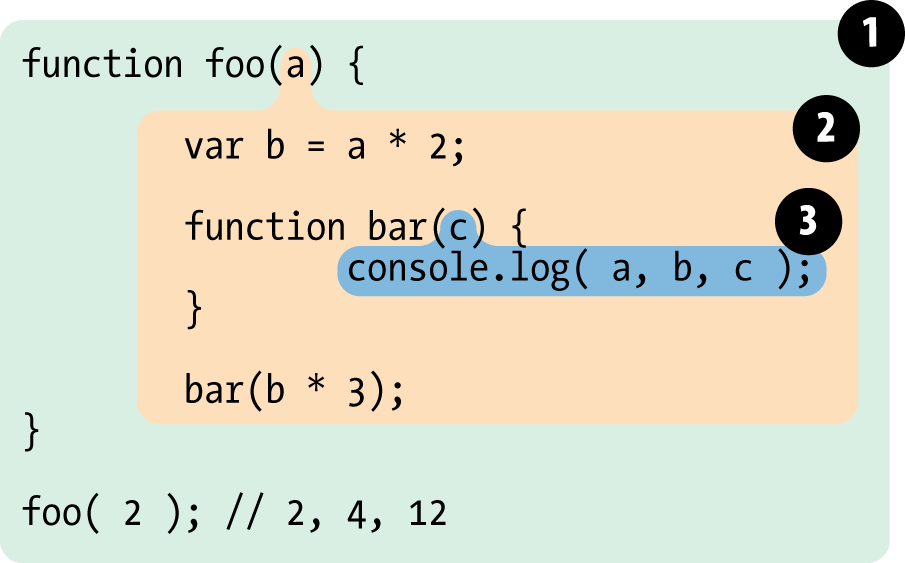
\includegraphics{fig2.png}
\caption{Scope as bubbles \cite{getify}}
\end{figure}

\section{Survey \& Interviews}\label{survey-interviews}

To form a general understanding of how IDEs and some of their specific
features are used, an online survey targeted towards professional
developers was created. The survey ran in April 2014 over the course of
two weeks and yielded answers from 45 participants.

Besides general questions, e.g. which programming languages and IDEs the
participants used, it collected information about the usage of the
following IDE functionalities:

\begin{itemize}
\itemsep1pt\parskip0pt\parsep0pt
\item
  Navigation of code
\item
  Debugging
\item
  Usage of API and language documentation
\item
  Autocompletion
\item
  Project structure and scaffolding
\item
  Asynchronicity
\item
  Syntax Highlighting
\end{itemize}

For each of the areas it was asked if and how the participants were
using them and—if appropriate—how their IDE was supporting them. They
survey instrumented multiple-choice questions with an additional „Other“
field for custom answers, as well as open-ended questions with a
free-form text field.

\chapter{Design Iterations}\label{design}

The following chapter exposes the design process and reasoning behind
the design decisions made for the prototypes. It leads through the
different prototyping stages and user testing, closing with an
evaluation of the design.

The prototyping happened in three subsequent stages. The first stage
comprised a set of pencil sketches on paper; the second prototype was
created with web technology, but fixed around a certain source code and
faked interactivity; the third prototype was implemented as a plug-in
for the Atom editor, called \emph{Scope Inspector}, and is able to work
with any source code it is provided.

In chapter \ref{exploration}, we developed four \textbf{characteristics}
of well-integrated language tools: performance, modularity, smartness,
and a focus on code. Additionally, we listed five common scoping
\textbf{problems} in chapter \ref{concepts}: hoisting, closure,
shadowing, implicit variable declaration, and lookup performance. The
design needs to address both the characteristics (non-functional
requirements) and the problems (functional requirements). For every
prototype, the addressed requirements are referred to in the respective
section. However, some requirements are not addressed at all. The
\emph{smartness} characteristic is not explicitly focused on by the
design, as in the case of scope there is no ambiguity. Neither is
\emph{Closure} addressed by any of the prototypes, for the reason that
it is—from a technology perspective—hard to \emph{correctly} detect. It
is certainly possible , but given the short amount of time it was not a
priority. Finally, linting tools already point out \emph{implicit
variable declaration}, which is why it is not in the scope of the
design.

\section{Definitions}\label{definitions}

To be able to discuss the qualitites of the concept and prototypes, we
must first define a number of terms.

\begin{description}
\item[Scope block]
In a JavaScript text file, a scope block is the textual block
representing a logical scope. For a function, which in JavaScript
creates a new scope, the scope block starts at the \texttt{function}
keyword and ends at the closing curly brace \texttt{\}} of the function
body. If, in a text editor, the cursor is placed anywhere inside this
scope block (but outside of child scopes), the scope block is called
\emph{active scope}.
\item[Current scope]
In a running JavaScript program, it is the currently executed scope.
This is a term related to the run-time rather then to author-time, and
should not be confused with \emph{active scope} described below.
\item[Active scope]
The scope which is currently in focus of editing. In relation to IDEs,
code editors and the prototypes presented in this chapter, the active
scope always describes the scope that the cursor is placed in.
\item[Local scope]
In the context of nested scopes, the local scope is the one in focus (be
it in the execution context during run-time, or the editing context
during author-time). Local scope is contrasted with non-local scope;
scopes that are logically distant from the local scope. Those may be
ancestor scopes, descendant scopes, or parallel scopes. The term is also
used to contrast \emph{global scope}.
\end{description}

\section{Sketching}\label{sketching}

One could argue that sketching is part of the earlier exploration phase,
rather than of the prototyping phase. However, next to sketching
different ideas, the author also sketched different possible
implementations for one feature that seemed valuable to the design
solution: \emph{highlighting}. Highlighting of scopes through different
colours—text or background colours—makes deeply nested scope more
visible and thus directly addresses the problem of \emph{lookup
performance}.

The basis for the sketches were printouts of the same source code, each
leading to a different way of highlighting.

\subsubsection{Active scope, inclusive}\label{active-scope-inclusive}

This sketch highlights the active scope block by applying a background
colour to it. The highlighting is \emph{inclusive}, i.e. any descendant
(inner) scopes are highlightes as well.

\subsubsection{Active scope, exclusive}\label{active-scope-exclusive}

Same as above, but descendant scope blocks are excluded from
highlighting. This way of highlighting was implemented in the scripted
prototype (see section \ref{working-prototype}).

\subsubsection{Active scope and ancestor
scopes}\label{active-scope-and-ancestor-scopes}

Next to highlighting the active scope, its ancestor scopes can also be
highlighted to emphasize nesting. To contrast the ancestor scopes from
the active scope, the highlighting would make use of different
background colours, for example different shades of grey. This way of
highlighting can be combined with both the inclusive and exclusive
approach.

\subsubsection{Scope colouring}\label{scope-colouring}

Described by Crockford \citeyear{crockford} as „context colouring“, this
way of highlighting would not apply a background colour, but instead
replace the existing forms of syntax highlighting. Thus, the
highlighting would not depend on the cursor position (which defines the
\emph{active scope}), but would be static instead.

\subsubsection{Identifier origin}\label{identifier-origin}

Additionally to emphasizing code blocks, individual identifiers can be
highlighted. Given a highlighted active scope, this sketch highlights
identifiers that are defined in that scope but used somewhere else (in
descendant scopes).

This works as well for the \emph{scope colouring} described above, as
each scope has a fixed colour. Identifiers that are used in other scopes
than they are defined in can therefore always be recognized if they
appear in the colour of their origin scope.

\begin{figure}[htbp]
\centering
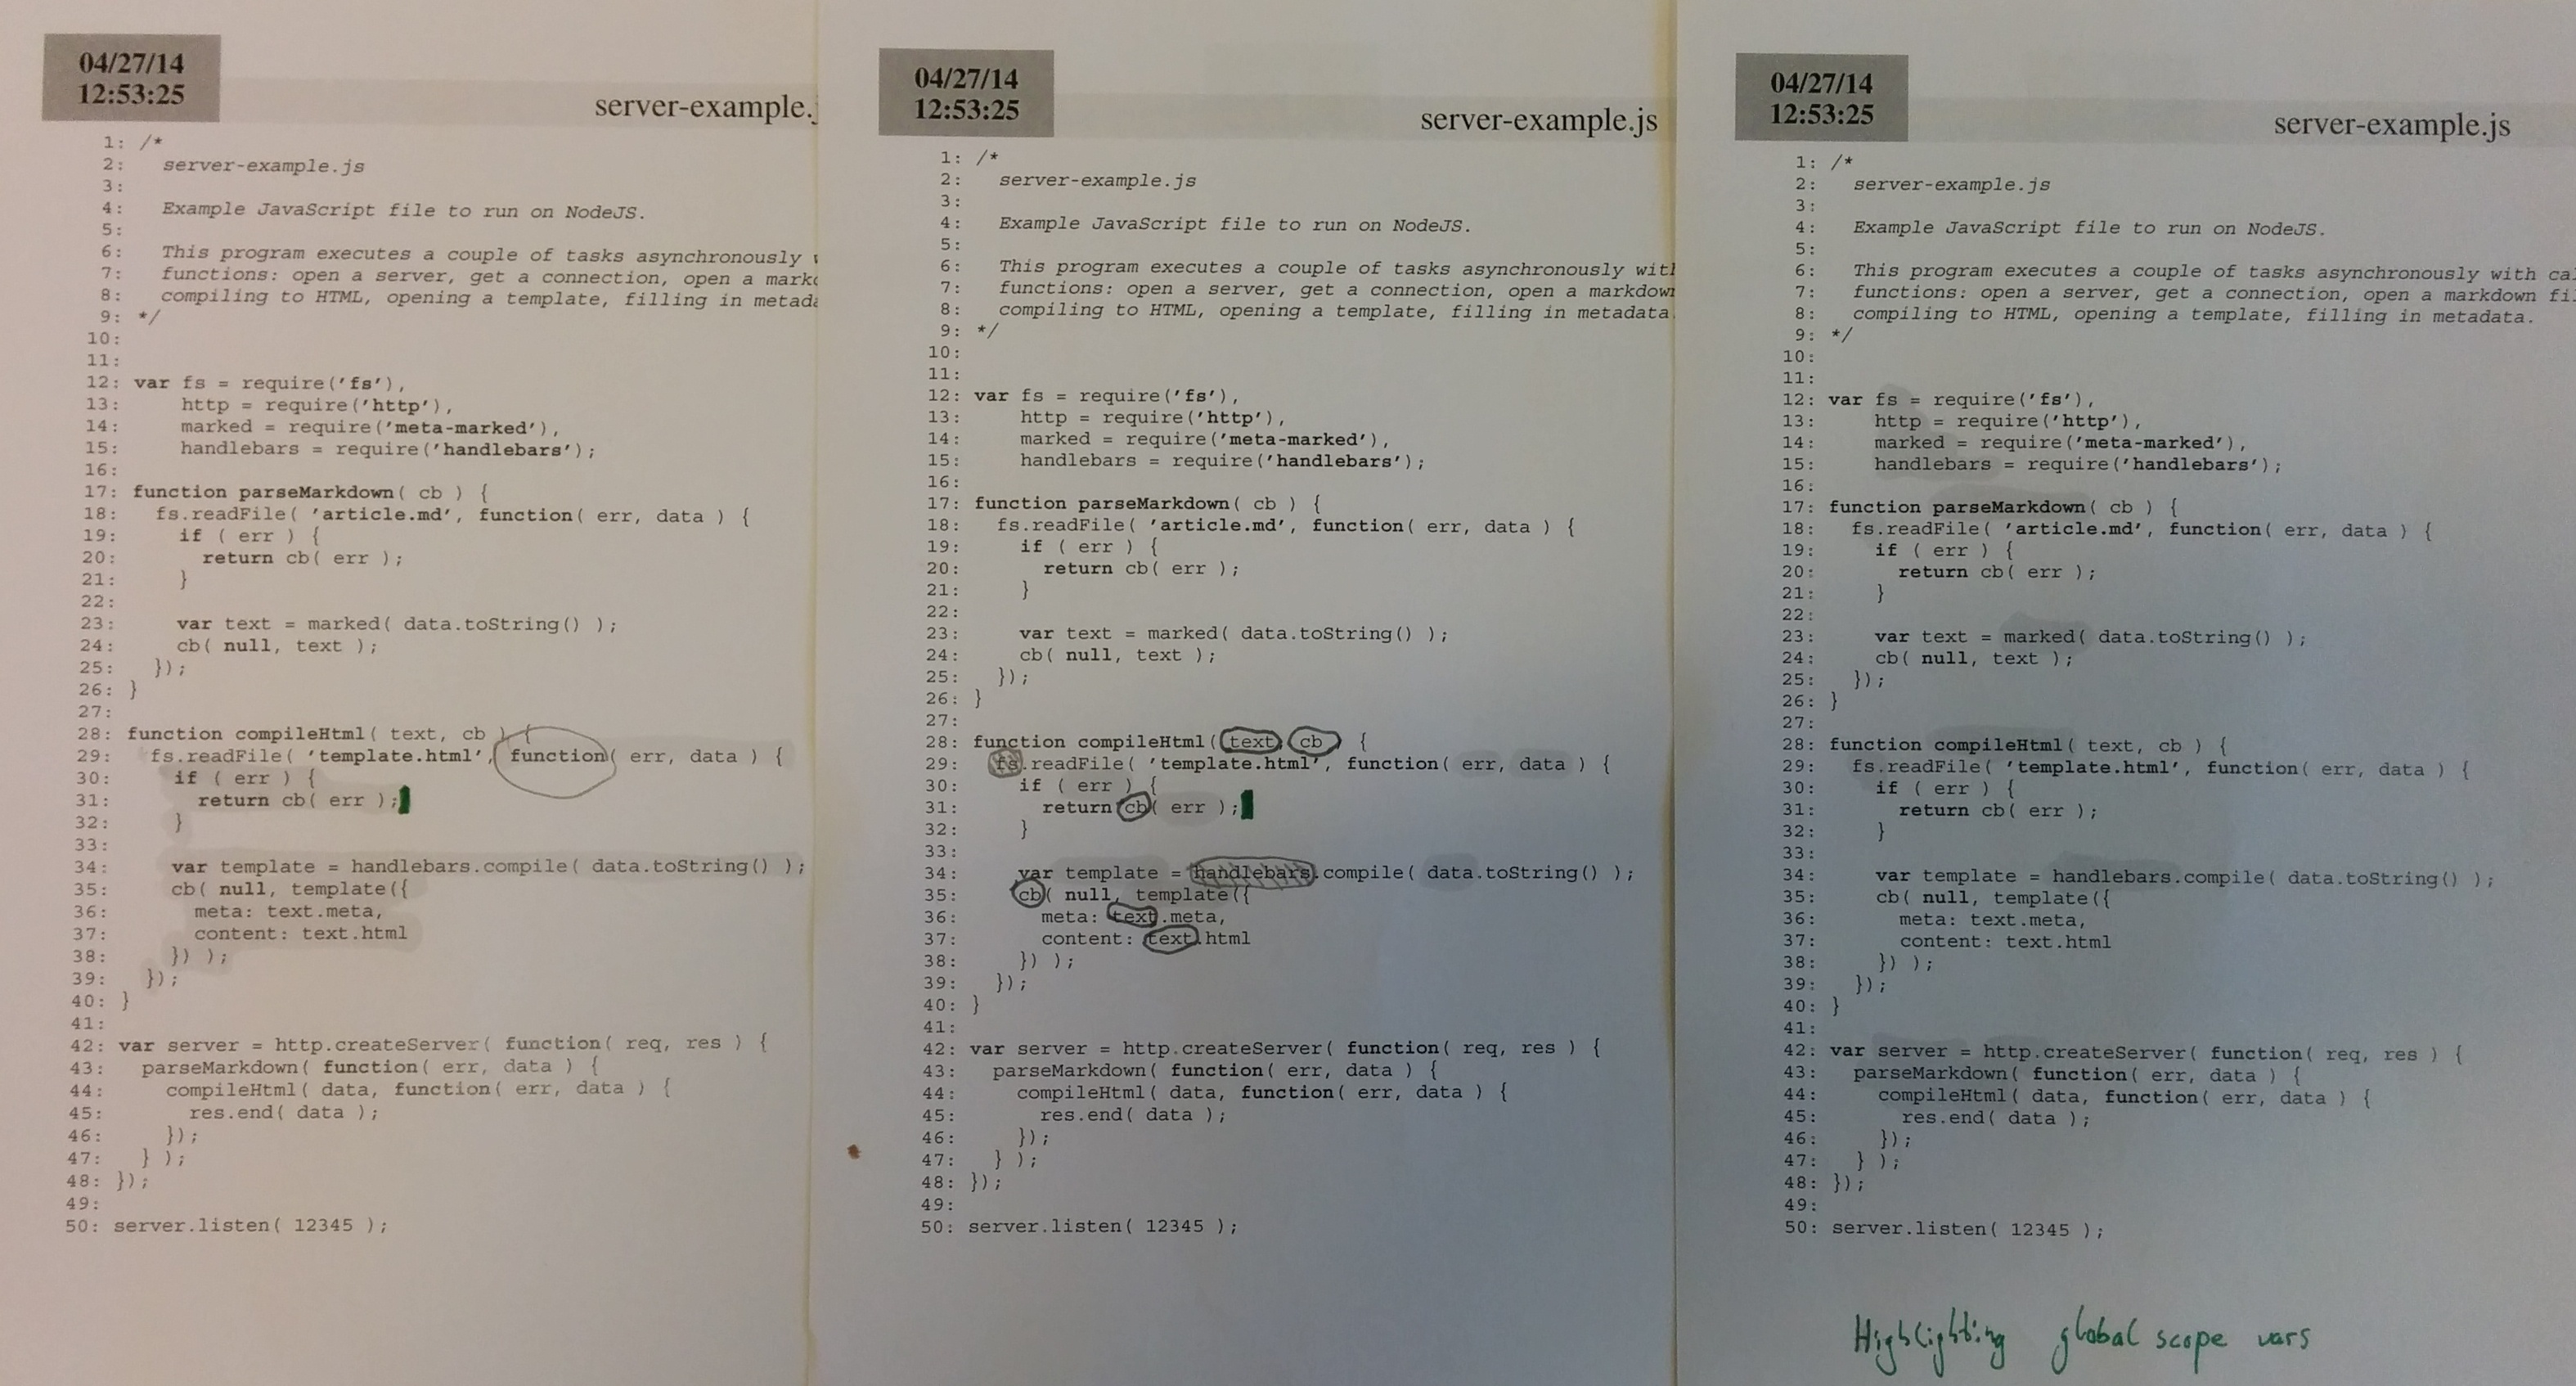
\includegraphics[keepaspectratio,width=\textwidth]{img/sketch_highlighting.jpeg}
\caption{Some of the sketches to explore ways of highlighting}
\label{fig:sketches2}
\end{figure}

\section{Scripted prototype}\label{scripted-prototype}

It very quickly became clear that the sketches were of little value.
Although most of them gave a general impression on where the selected
scope started and where it ended, it did not allow the user to see the
big picture. It seemed probable that a more interactive prototype would
be more helpful in this regard. As its capabilities of working with code
are limited and the code had to be specifically prepared, this is called
a \emph{scripted prototype}.

As the author is most familiar with web technologies, the scripted
prototypes would be built using \ac{html}, \ac{css} and JavaScript and
run in a web browser. Other prototyping tools, such as Balsamiq or
Indigo Studio, would not allow for enough detail in terms of
highlighting certain code passages, and would have represented a
learning overhead.

\begin{figure}[htbp]
\centering
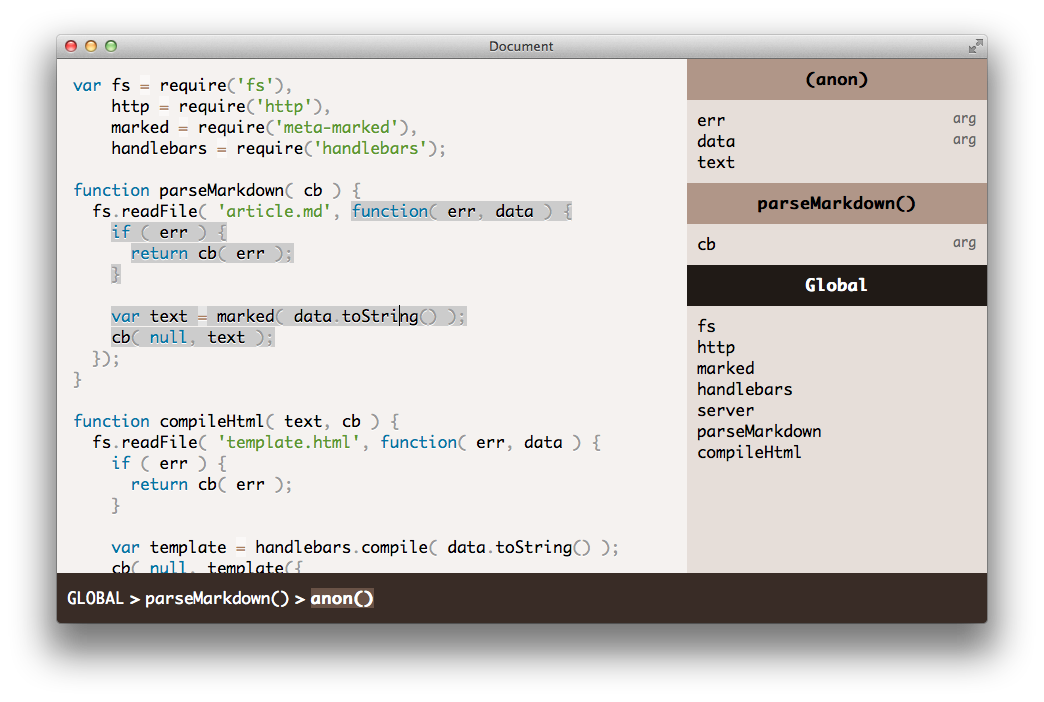
\includegraphics[keepaspectratio,width=0.75\textwidth,height=0.75\textheight]{img/prototype-1.png}
\caption{Screenshot of the scripted prototype run in a browser}
\label{fig:scriptedprototype}
\end{figure}

A code syntax highlighter\footnote{Prism, see \url{http://prismjs.com/}}
was used to turn the subject source code into styled \ac{html} tags, to
make it appear as if it was inside of a real code editor. Applying
syntax highlighting was also necessary to see if the different
highlighting techniques, as sketched out in the previous phase, would
interfere with syntax highlighting.

Furthermore, markers in the form of HTML tags were added to the subject
source code, which made it possible to apply different
styles\footnote{For example text colours, background colours, of font styles.}
to regions of the code. This was later used to realize highlighting of
the \glspl{scope-block}.

Two distinct \ac{ui} elements were added: a sidebar and a bottom bar.
The content of both depends on the \emph{active scope}, i.e. the scope
the cursor is placed in.

For each of the nested \ac{scope-block} that the cursor is positioned in
(beginning from the local scope, going outwards up to the global scope),
the sidebar shows a pane. Each pane contains the scope’s name along with
a list of identifiers defined within that scope. In opposition to the
working prototype, the scripted prototype does not show phenomena like
hoisting and shadowing. The panes are ordered ascending by logical
distance, i.e. the local scope would be on top, the next surrounding
scope beneath it, and so forth; up to the global scope on the bottom.

The different panes are hard-coded: all panes exist in the markup of the
prototype at all times and are pre-filled with the relevant data, but
are shown and hidden on demand.

The bottom bar shows a horizontal list of scope names. It makes use of
the \emph{breadcrumbs} \ac{ui}
pattern\footnote{In the Yahoo pattern library: \url{https://developer.yahoo.com/ypatterns/navigation/breadcrumbs.html}}.
Each listed scope, beginning from the global scope on the very left, up
to the local scope on the right, can be highlighted and navigated to by
clicking on its label. By
hovering\footnote{Hovering: Placing the mouse cursor over an element.}
over the label, the user can get a preview of the target scope, as it is
highlighted in the editor alongside the currently active scope.

\subsection{Constraints}\label{constraints}

The scripted prototype has some drawbacks, some of which might influence
its quality. The most obvious one is the fact that it only works with a
static, predefined source code, which is manually adapted to serve the
prototype’s purpose. This implies that

\begin{enumerate}
\def\labelenumi{\arabic{enumi}.}
\itemsep1pt\parskip0pt\parsep0pt
\item
  changes can not be made to the code, which makes the experience of the
  prototype very different from a real code editor, and
\item
  it is hard to tell if the prototype works similarily well with code
  that is more complex, less complex, or of an overall different style.
\end{enumerate}

The fact that there are no text editing facilities comes with another
drawback, namely the absence of a cursor. If a cursor cannot be placed
anywhere in the editor, the „activation“ of a scope block must be
achieved differently. In the case of this prototype, it is solved by
clicking on a piece of code. However, clicking anywhere in the line
besides the actual text will not change the active scope.

\subsection{Evaluation of the scripted
prototype}\label{evaluation-of-the-scripted-prototype}

The prototype was tested with two JavaScript developers in individual
in-person walkthrough sessions. The users were introduced to the
concept, if they were not familiar with it already, and explained the
basic constraints of the prototype (as mentioned above). They were
thereafter able to explore and test the prototype to their likings. One
of the two sessions have been recorded as a screencast.

The users liked both the „preview“ feature (hovering over a breadcrumb)
and the sidebar. The preview gave them an opportunity to quickly get a
visual overview of your position in the code and the active scope chain.
The sidebar showed them which variables and functions are available in a
given context. Overall, they liked the dynamicity of the prototype, as
they could „play around“ with it and understand the design concept just
by trying. They quickly made a connection between they position of the
cursor and the active scope along with its content.

One of the users suggested possible improvements or alternative designs
for existing features. He recommended a wider use of colour coding to
create a link between the scope in the editor window and the sidebar,
for example by colouring all the ancestor scopes in different shades of
grey. He also suggested an alternative visual structure for the sidebar
instead of the list, for example nested clusters or a graph. For
hoisting, the user came up with an idea to integrate indicators into the
text editor: a „phantom“ variable declaration, which would be grey and
not editable, could be inserted on top of a scope, to show that a
certain variable declaration would be hoisted up there. This indicator
should be collapsible so that it does not interfere with the editing
process. Because of technical constraints, this idea was not implemented
in the next prototype iteration; however, it seems a sensible solution
to the hoisting indication problem, as it communicates this implicit
phenomenon very clearly.

In conclusion, the prototype was well-received and served its purpose
well. It became clear that a consistent and clear visual language for
the next iteration of the prototype was necessary, and that a direct
connection between the code and the scope visualization has to be
communicated. Like the sketches, it addressed the \emph{lookup
performance} problem by visualizing nested scope, even more so through
the sidebar and bottom bar. It also put a stronger \emph{focus on code}
by making it navigatable using the bottom bar, and by dynamically
showing changes directly in the editor.

\section{Working prototype}\label{working-prototype}

The third and final prototype was built as a working prototype capable
of handling any JavaScript scope, rather than as a proof-of-concept. It
was integrated into the Atom\footnote{See \url{https://atom.io/}} text
editor as a so-called \emph{package} or \emph{plug-in}, released as
\gls{oss} and was made publicly available for using and testing. The
package is called „Scope Inspector“ and will be referred to using this
name throughout this section.

\subsection{The prototyping platform}\label{the-prototyping-platform}

For the prototype to yield meaningful results, I decided to integrate it
into a real \ac{ide}. This decision was informed by several
circumstances. The first and most obvious is that I could address a
broader community of users this way. If the prototype was, like the
scripted prototype, implemented in isolation as a standalone
application, it would raise the barrier for people to test and for me to
distribute it. But by building it as a plug-in to an existing \ac{ide},
I could leverage the distribution channels that were already in place. A
second reason is that users are already familiar with the software and
do not have to orientate themselves anew. This also implies that all the
features that the user \emph{expects} from an \ac{ide} are in place, and
the prototype can more seamlessly be integrated into the user’s
workflow. Finally, the third reason for building a prototype on top of
an existing \ac{ide} is that it can make use of the design language in
place, which eliminates the need to take decisions that are rather
irrelevant for this prototype, such as the choice of a typeface and
colour palette.

As a prototyping platform, the author decided on the Atom text editor.
Atom is open source and created by the software company Github. By the
time of writing, Atom is a relatively young project with a growing
community and plug-in ecosystem. The reasons for deciding in favour of
Atom are threefold: the technologies it is built upon, its internal
software architecture, and the user group it is targeting.

Atom is built on web technologies, namely
WebKit\footnote{See \url{http://www.webkit.org/}} and
Node.js\footnote{See \url{http://nodejs.org/}}. WebKit is the browser
engine used by the web browsers Google Chrome and Apple Safari, amongst
others, and is therefore responsible for the \acl{ui} layer of Atom.
Node.js is the JavaScript platform responsible for running any
non-\ac{ui} logic. Atom is mostly written in
CoffeeScript\footnote{CoffeeScript is a programming language that transcompiles to JavaScript.}.
Consequently, Atom packages can be written in CoffeeScript or
JavaScript, using HTML and CSS for the \ac{ui}. As I am familiar with
these technologies, Atom provided an ideal prototyping platform with a
low entry barrier.

For extending Atom, it offers an \ac{api} which can be used by plug-ins.
Atom’s internal architecture is built in a modular way, so that plug-ins
can hook into nearly everything that happens and react on it. The
prototype makes use of this fact in many ways, for example by showing
and hiding its \ac{ui} elements depending on the type of file that is
being edited. In general

Atom is marketed by Github as a „hackable text editor for the 21st
Century“\footnote{See \url{https://atom.io/}, accessed 18.05.2014}. It
is also intended to be a „deeply extensible system that blurs the
distinction between ‚user‘ and ‚developer’.“ Those claims lead to the
conclusion that Atom is a text editor built for developers,
especially—but not exclusively—web developers. While not every web
developer is a proficient JavaScript developer, the target groups of
Atom and this prototype seem to overlap to a large extent.

\subsection{Parsing and gathering relevant
information}\label{parsing-and-gathering-relevant-information}

For the prototype to be as \emph{complete} and \emph{correct} as
possible, it was built on top of an existing JavaScript parser called
Esprima\footnote{See http://esprima.org/}. The process of extracting the
relevant scope structure and annotations from the
\ac{ast}\footnote{The \ac{ast} is the data structure that is returned by the parser, which contains all the lexical statements and expressions.}
will not be discussed here in greater detail, but is instead described
in a blog post \cite{tvo}.

However, it is important to mention what data structures are extracted
from the source code. Analoguous to the nature of JavaScript scope as
described in chapter \fullref{research}, the data structure is a
hierarchy of objects. Each object represents a scope and may have
metadata as well as a list of identifiers attached to it. An identifier
is either a child scope (as created by a function) or a variable. For
scope objects, the metadata are its name and its location in the source
code (row and column of the start and end points), whereas for variables
the metadata are its name, location, if it is hoisted, by which child
scope identifiers it is shadowed, and which identifier it is shadowing.

A diagram of an exemplary data structure is shown in figure
\ref{parser}.

\textbf{TODO: insert diagram of data structure here}

Using this data structure, the prototype can show meaningful data to the
user, which would not have been possible with the \ac{ast} alone. The
modular composition of the prototype, which decouples the task of
parsing from the task of displaying information, makes it possible to
re-use each of the components. The component described in this section,
which is responsible for turning the \ac{ast} into a „scope tree“, could
be used in plug-ins for any \ac{ide} to achieve similar functionality as
the one of this prototype.

\subsection{Interface and
Interactions}\label{interface-and-interactions}

The design respects that the subject of a developer’s work is the code
itself, not the tools that surround it. This is why the solution
integrates into the most important part of the IDE, the text editor,
directly. The features built into the editor itself will be called
\emph{inline} features.

Atom’s interface is, by default, threefold: the text editor takes the
most space; on its left is a sidebar containing a file browser, and on
the bottom is a status bar. As many web browsers, text editors, and
IDEs, multiple open files are accessed through \emph{tabs} on the top of
the screen. The tabs are important, because the Scope Inspector will
only be active as long as an editor with a JavaScript file is in the
foreground. Whenever the user switches to another tab, the Scope
Inspector is activated or deactivated, depending on if the tab contains
an editor with a JavaScript file or not.

Throughout the Scope Inspector package, a visual style consistent with
Atom’s is used. Any icons in use are taken from the
Octicons\footnote{See \url{https://github.com/styleguide/css/7.0}} icon
set, which is incorporated into every Github product. Atom supports
themes (colour schemes) for both the application window and the editor.
Scope Inspector makes use of the colours defined in those themes. This
way, the package \ac{ui} feels more natural to the user. However, there
may be difficulties if the theme is not well-defined and the colours are
badly balanced. One user reported very low contrast between the editor’s
background and the scope highlighting. In addition to pre-defined theme
colours, Atom also provides a set of pre-styled \ac{ui} components, for
example buttons and panes, which have been used in the prototype.

Whenever the Scope Inspector is active, two things are obvious: on the
bottom of the editor, a panel is shown which we call \emph{bottom bar},
and the active scope is highlighted inline. Additionally, a sidebar can
be toggled using the Atom command „Scope Inspector: Toggle Sidebar“.
This command is accessible using the menu, the command palette, a
keyboard shortcut (\texttt{Ctrl+Alt+i} by default), and a toggle button
on the bottom bar. The user can choose wether or not to use the package
with the sidebar enabled, which addresses the \emph{modularity}
characteristic. For \emph{performance} reasons, the JavaScript program
is not re-evaluated (i.e. its scope structure is built up) on every
character that is typed by the user, but only when its file is saved.
The several components and their functionality are explained in more
detail in the following sections.

\subsubsection{Inline scope
highlighting}\label{inline-scope-highlighting}

As explained above, the \emph{active scope} is the immediate scope the
cursor is placed in. It is emphasized by highlighting it through a
lighter or darker background colour (depending on Atom’s colour scheme).
If the cursor is placed in a different scope, the formerly active scope
is de-highlighted, and the now active scope is highlighted instead.

\begin{figure}[htbp]
\centering
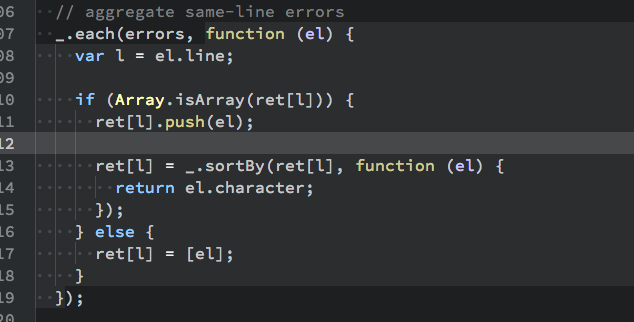
\includegraphics[keepaspectratio,width=0.75\textwidth]{img/scope-highlight.png}
\caption{Subtle highlighting of an anonymous function}
\label{fig:protohighlighting}
\end{figure}

While the scripted prototype implements \emph{exclusive highlighting},
the working prototype implements \emph{inclusive highlighting}, which
means that the inner scopes are highlighted as well. This is due to
technical reasons; building exclusive highlighting into the prototype
would have taked a lot more time. In further iterations of the
prototype, an option to enable and disable exclusive highlighting could
be provided.

The bottom bar contains a toggle
button\footnote{A switch in the form of a button, which can be either \emph{on} or \emph{off}.}
to enable or disable highlighting of the global scope. Highlighting the
global scope with \emph{inclusive highlighting} is not useful, as the
whole file would be highlighted (and there would be nothing left to
contrast the highlight to).

\subsubsection{Inline hosting
indication}\label{inline-hosting-indication}

If there are identifiers being hoisted in the active scope, an
indicator—which consists of a dotted line with an arrow head—is shown
inline. The indicator appears at the place in the source code where the
identifiers are hoisted to. This is \emph{before} the first statement in
the given scope which is not a variable declaration. In figure
\ref{protohoisting}, this is before the very first line of the scope
block. By hovering over the indicator line, the user reveals a tooltip
listing all the identifiers that are being hoisted to this place. This
feature obviously addresses the \emph{hoisting} problem, and does so
while maintaining a \emph{focus on code}.

\begin{figure}[htbp]
\centering
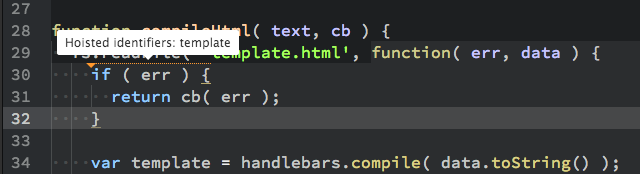
\includegraphics[keepaspectratio,width=0.75\textwidth]{img/hoisting.png}
\caption{Inline hoisting indicator with tooltip}
\label{fig:protohoisting}
\end{figure}

\subsubsection{Bottom bar}\label{bottom-bar}

The bottom bar serves two purposes: it provides a quick glance of where
in the scope hierarchy the cursor is and provides quick access to two
settings.

\begin{figure}[htbp]
\centering

\includegraphics[keepaspectratio,width=0.75\textwidth]{img/bottombar.png}
\caption{The bottom bar, showing the scope chain and toggle buttons}
\label{fig:bottombar}
\end{figure}

On the right side of the bottom bar, two toggle buttons allow for
enabling and disabling of two features. The right button, showing a list
icon, shows or hides the sidebar. The left button with the label
„Highlight Global“ toggles the highlighting of the global scope (as
described above).

The left side of the bottom bar shows the breadcrumbs known from the
scripted prototype. The breadcrumbs, implemented as simple buttons, are
labeled with the corresponding scope name. The global scope is always on
the left, whereas the currently local, active scope is on the right. By
hovering over any of the breadcrumb buttons, the user can preview the
respective scope highlighting in the editor. The preview is applied in
addition to the currently active highlight in a different colour.

By hovering over the breadcrumbs from left to right or from right to
left, the user can make the relationship between the logical structure
of the JavaScript program (in the form of hierarchic scopes) and the
textual structure (in the form of code) visible. As in the previous
prototype, the bottom bar emphasizes the scope nesting and thus
addresses the \emph{lookup performance} problem.

\subsubsection{Sidebar}\label{sidebar}

The sidebar shows content depending on the currently active scope.
Similarily to the scripted prototype, the sidebar lists one pane for
each scope in the hierarchy of the active scope. The active scope is
listed on top, while its ancestors are listed below, up to the global
scope on the very bottom.

\begin{figure}[H]
\centering
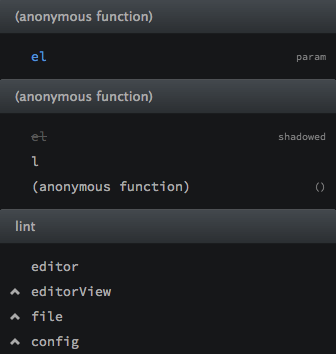
\includegraphics[keepaspectratio,width=0.4\textwidth]{img/sidebar.png}
\caption{Sidebar (clipped), with shadowing, shadowed, and hoisted identifiers}
\label{fig:protosidebar}
\end{figure}

Each pane is entitled by the name of the scope. In case of function
scope, the name of the function becomes the scope name („(anonymous
function)“ in the case of an unnamed function expression). In case of
the global scope, the name is „GLOBAL“. Underneath the title, the names
of all identifiers defined within the scope are listed, along with
certain attribute annotations.

\begin{itemize}
\itemsep1pt\parskip0pt\parsep0pt
\item
  Function parameters are listed first. They appear with the annotation
  „param“, set in smaller text size to the right.
\item
  General variables follow the parameters. If they are not shadowed,
  they have no annotations.
\item
  Functions are the last entities in the list. They are connotated with
  a pair of parantheses „()“.
\end{itemize}

The listed identifiers show also if they are hoisted, shadowed, or if
they shadow other identifiers. This is indicated by different stylistic
changes.

\begin{itemize}
\itemsep1pt\parskip0pt\parsep0pt
\item
  Hoisted identifiers have a small, upwards-pointed arrow on the left
  side of their label. This indicates that their declaration is
  implicility moved upwards in code.
\item
  Shadowed identifiers are printed in a more subtle text colour. Besides
  that, their label is striked-through to indicate that they are not
  accessible within the given descendant scope.
\item
  Identifiers that shadow other identifiers in ancestor scopes are
  printed in a highlight colour. In case of Atom’s standard \ac{ui}
  theme, this is a bright blue colour.
\end{itemize}

Consequently, the sidebar addresses both the \emph{shadowing} and
\emph{hoisting} problems.

\section{User Testing \& Evaluation}\label{user-testing-evaluation}

The goal of user testing was to collect both qualitative and
quantitative data through different methods. The quantitative data
collection was built into the prototype in form of a connection with
Google Analytics\footnote{A website and app analytics platform.}.

\subsection{Test installment}\label{test-installment}

Atom includes a package management system with an online repository,
called \ac{apm}. This system allows any developer to publish Atom
packages and thus make them available for any Atom user to download and
use. Consequently, this prototype was distributed via \ac{apm}.

The author was collaborating with two full-time developers and one
part-time developer. They agreed to install the package and use it over
the course of one week (full-time developers) or one day (part-time
developer), respectively, integrating it into their usual workflows.

\begin{itemize}
\itemsep1pt\parskip0pt\parsep0pt
\item
  2 inquiries
\item
  hintergrund der thesis erklären
\item
  klar machen dass dev weiß wie scope funzt
\end{itemize}

In addition to this directed user test, publishing the prototype via
\ac{apm} made it available to the general public. It was announced on
several social networks, especially targeting existing Atom users, with
the goal of getting users to download and use it. A week after
publishing the prototype, the number of downloads counted ???. This way
of testing „in the wild“ makes it harder to gather feedback, compared to
the method of addressing potential users directly. However, the
analytics mechanism built into the prototype yielded quantitative data
for evaluation.

\subsection{Usage metrics}\label{usage-metrics}

The prototype was built with the option to collect usage metrics using
the Google Analytics service. By default, this option was set to
\emph{off}, as I oppose the unknown tracking of any data for ethical
reasons. However, users were asked in the \texttt{README} file, which is
displayed both on the package’s
page\footnote{See \url{https://atom.io/packages/scope-inspector}} and on
Github\footnote{See \url{https://github.com/tvooo/scope-inspector}}, to
enable tracking in Atom’s \emph{settings} panel for the Scope Inspector
package.

If enabled, the following events are tracked:

\begin{itemize}
\itemsep1pt\parskip0pt\parsep0pt
\item
  The package is enabled/disabled
\item
  The sidebar is shown/hidden
\item
  The user hovers over a scope breadcrumb in the bottom bar and thus
  previews a scope highlighting
\item
  The user clicks on a scope breadcrumb in the bottom bar and thus jumps
  to the beginning of scope, making it the active scope and highlighting
  it
\end{itemize}

Through collecting these events, a claim can be made—to a certain
extent—for how helpful certain features are.

\subsection{Testing Results}\label{testing-results}

\subsubsection{Analytics}\label{analytics}

Analytical metrics have been tracked over the course of 13 days. In
total, five different users (including myself) had tracking enabled,
with a peak of fours simultaneous users. On average, two to three users
contributed data each day.

In those nearly two weeks, the sidebar was enabled 76 times, whereas
interactions with elements on the bottom bar happened 144 times.
However, only 22 of those interactions were clicks which have to happen
intentionally—the hover events can occur by chance (for example by
moving the mouse from the editor window to the status bar and
vice-versa). Given those circumstances, it can be concluded that the
sidebar was more in use than the bottom bar. But event metrics can not
measure if users used the bottom bar for orientation, for example just
by looking at it and figuring out where in the scope hierarchy they are.
Thus, the analytics result are of limited use for the evaluation of the
prototype.

\subsubsection{Interviews with
developers}\label{interviews-with-developers}

This section summarizes the finding of the user testing, as collected
through interviews. None of the interviewees had used the prototype
before, and both are only casual Atom users.

\begin{description}
\item[Inline]
The inline highlighting was perceived as useful, as users claimed it
helped them to focus on the current code and also showed them the scope
limits (in code). None of the developers discovered the inline hoisting
indicator, it had to be pointed out to them. Even after pointing it out,
the users did not use the inline indicator, but instead just looked at
the sidebar to see which identifiers were being hoisted. One of the
developers was not familiar with the concept of hoisting.
\item[Sidebar]
One functionality that each user found to be missing was a means of
navigation through the sidebar. Two users expected to be able to jump to
a variable declaration if he sees a problem there, just by clicking on
the variable’s name. Another user thought the ability to scroll to a
certain variable was denoted by the upwards pointing arrow next to it.
It was also suggested to be able to jump to the beginning of a scope by
clicking on its respective headline, similar to what happens when the
user clicks a breadcrumb in the bottom bar. Adding line numbers for each
identifiers was also suggested, in order to be able to distinguish
anonymous functions better from each other.

The order of the panels, each representing one scope in the scope chain,
was confusing to some users. Although they understood the concept of a
scope chain, they expected it to be in the order that scopes appear in
code. However, code is linear, while scope is hierarchical, and they do
not map directly. It is reasonable to assume that the order which is
used in the prototype is learnable for the users, as it works
analogously to \ac{css} in the Chrome DevTools. This could for example
be achieved by connecting the scope in the sidebar visually with its
counterpart in the editor. One user suggested that, when a scope is
hovered in the sidebar, its counterpart in the editor could be
highlighted (analogous to the effect of hovering a breadcrumb in the
bottom bar).

Another suggestions concerning the sidebar was to highlight even single
variables in the editor when they are highlighted in the sidebar.
Regarding shadowing, one user was able to detect a bad practice in his
code during testing: he had created a shadowing situation in which the
two variables of the same name server completely different purposes.
Another user misinterpreted the hoisting indicators (upwards arrows) in
the sidebar. He assumed that they are pointing upwards because clicking
on them would cause the editor to scroll upwards, navigating to the
identifier’s declaration.
\item[Bottom bar]
None of the users discovered on their own the possibility to navigate
the scope chain by clicking on the breadcrumbs. However, after pointing
the feature out, they stated it was useful. One user noted that, once
you navigate into a higher scope, you can not go „back“ to the last
position (or the previously selected scope, which is nested inside the
now active scope).

Two users stated that the bottom bar would take up too much space, as
most developers would like as much space as possible for their code.
They suggested to style the breadcrumbs more like hyperlinks on the web,
and also to indicate that they are breadcrumbs by deparating them
through rightwards pointed arrows. One user even suggested to get rid of
the bottom bar completely, in case that the sidebar would take its tasks
of navigating and previewing the scope chain.
\item[Modularity]
One of the users asked if he could disable the inline highlighting
altogether, as he could imagine it to be annoying in the long run; this
is not possible in the final prototype, as during the design phase the
highlighting was considered a central element of the design. He
suggested that all three parts of the prototype—inline highlighting,
sidebar, and bottom bar—should be optional.
\item[Miscellaneous]
Various comments concerned none of the areas above. A suggested feature
was for the prototype to give an overview of all the identifiers that
are affected by shadowing or hoisting, in order to quickly uncover
possible code smells. In general, so thought one user, would it be a
good idea to communicate the \emph{meaning} of a detected code smell and
show them how to interpret it: Why is it a possible defect, and what can
the developer do to fix it? This would be especially useful for more
comples findings, such as closures (which are not implemented in this
prototype). Those suggestions drive the design more into an educative
direction. Additionally, one bug was found during testing, which is
related to the parser and therefore not relevant to the interface.
\end{description}

In total, the prototype did well in user testing. Users stated that it
was unobtrusive and helpful, especially the highlighting and sidebar.
However, the bottom bar was not as useful to the developers, which
mirrors the quantitative results.

\subsubsection{Social Media Feedback}\label{social-media-feedback}

In the open source software community, social media channels are
frequently used to state an opinion on new products, to share news, and
to give feedback. The prototype, in the form of the Scope Inspector
package for Atom, received some positive feedback on different channels.

On Twitter, which was used as a marketing instrument as well, the
feedback was exclusively positive. One user called it „another reason to
consider switching from {[}Sublime Text to
Atom{]}“\footnote{See \url{https://twitter.com/adardesign/status/466589449561055232}},
while others seemed to be interested as
well\footnote{See \url{https://twitter.com/raganwald/status/466930480517246976}}.
Five tweets mentioning the package have been both retweeted and
favourited about 20
times\footnote{Based on tweets that could be found by the Twitter search for the keyword ```scope inspector’’’.}.

On the news platforms EchoJS and Reddit (JavaScript section) the package
got little attention: four and eight upvotes, respectively, although the
only comment on Reddit claims that it „looks
promising“\footnote{See \url{http://www.reddit.com/r/javascript/comments/25k30l/javascript_scope_inspector_an_atom_package_to/chi27cm}}.

On Github, users filed two issues (bugs). One user requested the
possibility to investigate identifiers in the sidebar more deeply (which
is impossible to do correctly if the program is not executed). The other
one asked for on-the-fly re-evaluation of the scope, as was already
asked for in the interviews. At the stage of the prototype, scope is
only re-evaluated when the file is saved; however, looking at linting
tools, re-evaluating a short time (100-200ms) after the user stopped
typing seems to be a promising
strategy\footnote{See \url{https://github.com/tvooo/scope-inspector/issues/7}}.
This method would have been tested in terms of performance.

Several
reactions\footnote{See \url{http://www.echojs.com/comment/9867/1} and \url{https://twitter.com/vilmosioo/status/466934333681717248}}
on the blog post about the technical side of the Scope Inspector
\cite{tvo} suggest that there are difficulties for JavaScript developers
to deal with CoffeeScript code. In other words, the target users of the
package (JavaScript developers) are not directly able to improve on or
modify the package itself. This complicates code contribution for this
open source project.

\chapter{Conclusion, Reflection}\label{conclusion-reflection}


%\newpage
\newpage
\thispagestyle{empty}
\mbox{}
\newpage
 %neue Seite, damit Link auf Seitenanfang zeigt
%\phantomsection %notwendig, damit Link nicht unterhalb der Überschrift zeigt
%\addcontentsline{toc}{chapter}{Bibliography} %Eintrag im Inhaltsverzeichnis



\bibliographystyle{agsm}
\phantomsection
\setcounter{page}{1}
\pagenumbering{Roman}
\addcontentsline{toc}{chapter}{Bibliography}
\bibliography{thesis}

% Uncomment to enable list of figures

%\newpage
%\setlength{\cftparskip}{-0.8pt}
%\phantomsection
%\addcontentsline{toc}{chapter}{List of Figures}

% don't uncomment the following two lines, for whatever reason
%\setlength\cftbeforechapskip{4pt}
%\setlength\cftbeforefigskip{4pt}

%\listoffigures

% Uncomment to enable list of tables

%\newpage
%\thispagestyle{empty}
%\mbox{}
%\newpage
%\newpage
%\phantomsection
%\addcontentsline{toc}{chapter}{List of Tables}
%\listoftables

% Uncomment to enable list of listings

% \newpage
% \listoflistings
% \addcontentsline{toc}{chapter}{List of Listings}

% Uncomment to enable glossary

% \newpage
% \printglossary{}

% Uncomment to enable appendix

%\chapter*{Appendix}
%\renewcommand*{\chaptermarkformat}{}
%\renewcommand*{\sectionmarkformat}{}
%\chaptermark{Appendix}
%\sectionmark{Appendix}
%\addcontentsline{toc}{chapter}{Appendix}
%\subsubsection*{Sample source code}
\label{app:diagram}
The following source code has been used for sketching during ideation and during prototyping.

\begin{listing}[H]
\begin{minted}[linenos=true,frame=none]{javascript}
;(function( window, document, $, undefined ) {
  console.log( this );
  $( document ).ready( function() {
    console.log( this );
    $('#btn').on('click', function( event ) {
      console.log( this );
      event.preventDefault();
      $.getJSON('document.json', function( data ) {
        console.log( this );
        data.forEach( function ( entry ) {
          console.log( this );
          $('#list').append('<li>' + entry.title + '</li>');
        });
      });
    });
  });
}( window, document, jQuery ));
\end{minted}
\caption{Sample client-side JavaScript program}
\label{lst:client}
\end{listing}

\begin{listing}[H]
\begin{minted}[linenos=true,frame=none]{javascript}
var fs = require('fs'),
    http = require('http'),
    marked = require('meta-marked'),
    handlebars = require('handlebars');

function parseMarkdown( cb ) {
  fs.readFile( 'article.md', function( err, data ) {
    if ( err ) {
      return cb( err );
    }

    var text = marked( data.toString() );
    cb( null, text );
  });
}

function compileHtml( text, cb ) {
  fs.readFile( 'template.html', function( err, data ) {
    if ( err ) {
      return cb( err );
    }

    var template = handlebars.compile( data.toString() );
    cb( null, template({
      meta: text.meta,
      content: text.html
    }) );
  });
}

var server = http.createServer( function( req, res ) {
  parseMarkdown( function( err, data ) {
    compileHtml( data, function( err, data ) {
      res.end( data );
    });
  } );
});

server.listen( 12345 );
\end{minted}
\caption{Sample server-side JavaScript program}
\label{lst:server}
\end{listing}


\end{document}
